% =====================================================================
%  ADDITIONS FOR RESULTS SECTION
%  Insert after the JAAD results discussion (after Fig.~\ref{fig:early}
%  or the dashboard figures) and before \section{Conclusion...}.
%  All numbers are from leak-free evaluations produced by the pipeline.
% =====================================================================

\subsection{Cross-Dataset Validation on PIE}

To test whether the pipeline generalises beyond a single benchmark, the entire
leak-free 5-fold cross-validation was repeated on the PIE (Pedestrian Intention
Estimation) dataset~[15], a larger and independently collected corpus. A
three-route subset comprising \textbf{228 pedestrian tracks} was used; every
track is evaluated exactly once and the out-of-fold predictions are pooled,
yielding \textbf{12{,}597 observe$\rightarrow$predict windows (611 crossing, a
4.9\% positive rate)}. The identical trajectory / pose / fusion ablation is
reported in Table~\ref{tab:ablation_pie}, using the same track-level splitting,
window geometry, and common-recall protocol as on JAAD.

\begin{table*}[t]
\centering
\caption{Feature-set ablation on \textbf{PIE} (RTMPose keypoints), leak-free
5-fold CV, 12{,}597 pooled test windows (611 crossing), common recall 0.58.}
\label{tab:ablation_pie}
\begin{tabular}{lccccc}
\hline
Feature set & AUC & AP & Balanced Acc. & F1 & AUC (mean$\pm$std) \\
\hline
Trajectory only (before)    & 0.684 & 0.131 & 0.669 & 0.184 & 0.719 $\pm$ 0.111 \\
Body-language only          & 0.786 & 0.160 & 0.709 & 0.243 & 0.787 $\pm$ 0.070 \\
Pose $+$ trajectory (after) & \textbf{0.797} & \textbf{0.228} & \textbf{0.709} & \textbf{0.243} & \textbf{0.806 $\pm$ 0.078} \\
\hline
\end{tabular}
\end{table*}

The fusion model again dominates. ROC-AUC rises from \textbf{0.684} for the
trajectory-only signal---which corresponds to the conventional
detection-plus-tracking (YOLO$+$ByteTrack) paradigm without behavioural
cues---to \textbf{0.797} for the pose$+$trajectory fusion, and average precision
increases from 0.131 to 0.228. On PIE the effect of body language is even more
pronounced than on JAAD: the pose-only model (AUC 0.786) already surpasses the
trajectory baseline by a wide margin, indicating that in the more varied and
less curated PIE scenes the crossing decision is carried more strongly by
posture and gait than by bounding-box motion alone. The lower 5-fold variance of
the pose-based models ($\pm$0.070 and $\pm$0.078, versus $\pm$0.111 for
trajectory) further shows that the body-language cues yield a more stable
estimator across folds.

Two points are important when comparing PIE against the JAAD results of
Table~\ref{tab:ablation}. First, PIE's crossing base-rate (4.9\%) is roughly five
times lower than JAAD's (23.6\%); since average precision is bounded below by the
positive rate, PIE's absolute AP (0.228) must be read against a no-skill floor of
0.049---i.e.\ the fusion model exceeds chance AP by $\approx$4.7$\times$, a larger
relative margin than on JAAD. Second, the threshold-free ROC-AUC, which is
insensitive to this base-rate difference, is in fact \emph{higher} on PIE (0.797)
than on JAAD (0.781). Table~\ref{tab:crossdataset} summarises this cross-dataset
comparison for the fusion model. Together these results confirm that the
data-cleaning-plus-spatio-temporal pipeline is not tuned to a single Western
benchmark but transfers to an independently collected dataset.

\begin{table}[t]
\centering
\small
\setlength{\tabcolsep}{4pt}
\renewcommand{\arraystretch}{1.15}
\caption{Cross-dataset generalisation of the pose$+$trajectory fusion model
(leak-free 5-fold CV). AUC is threshold-free and directly comparable; F1 and
balanced accuracy are reported at each dataset's baseline operating recall, and
AP scales with the dataset's crossing base-rate (noted).}
\label{tab:crossdataset}
\begin{tabular}{|l|c|c|c|c|c|}
\hline
\textbf{Dataset} & \textbf{Pose} & \textbf{Tracks} & \textbf{Windows (+ve \%)} & \textbf{AUC} & \textbf{AP} \\
\hline
JAAD & YOLO-pose & 190 & 2{,}528 (23.6\%) & 0.781 & 0.476 \\ \hline
PIE  & RTMPose  & 228 & 12{,}597 (4.9\%) & \textbf{0.797} & 0.228 \\ \hline
\end{tabular}
\end{table}

\subsection{Pose-Estimator Upgrade: YOLO-Pose to RTMPose}

The 17-keypoint estimator of the pose stage (S6) was upgraded from the initial
YOLO-pose (nano) model to a top-down \textbf{RTMPose} estimator, which is applied
directly to each pedestrian box and is markedly more robust on small, distant,
and partially occluded pedestrians. Because both estimators emit the same
17-keypoint COCO skeleton, the body-language feature layer of
Table~\ref{tab:features} is unchanged---only keypoint quality differs. Evaluated
on the identical held-out PIE split (seed 42, 1{,}564 windows, 109 crossing), the
fraction of pedestrian frames yielding usable keypoints rose from \textbf{72\% to
88\%}, recovering the small/occluded pedestrians the nano model silently dropped.
This lifts the threshold-free metrics of the pose$+$trajectory model
substantially, as shown in Table~\ref{tab:pose_backend}.

\begin{table}[h]
\centering
\small
\setlength{\tabcolsep}{4pt}
\renewcommand{\arraystretch}{1.15}
\caption{Effect of the pose-estimator upgrade on the pose$+$trajectory model
(PIE, held-out single split, seed 42, 1{,}564 windows). AUC and AP are
threshold-free; recall/F1 are at the recall-calibrated operating point.}
\label{tab:pose_backend}
\begin{tabular}{|l|c|c|c|c|c|}
\hline
\textbf{Pose model} & \textbf{Valid kpts} & \textbf{AUC} & \textbf{AP} & \textbf{Recall} & \textbf{F1} \\
\hline
YOLO-pose (nano)     & 72\% & 0.816 & 0.268 & 0.890 & 0.231 \\ \hline
RTMPose (top-down)   & \textbf{88\%} & \textbf{0.844} & \textbf{0.331} & \textbf{0.908} & 0.227 \\ \hline
\end{tabular}
\end{table}

RTMPose improves ROC-AUC from 0.816 to \textbf{0.844} and average precision from
0.268 to \textbf{0.331} while also increasing recall (0.890 to 0.908); the
essentially unchanged F1 reflects only the recall-oriented operating point, at
which the extra recovered detections trade a small amount of precision. The pose
stage nonetheless remains lightweight: the exported predictor is a 216\,KB NumPy
model running at $\approx$243 windows/s, preserving the edge-deployability
targeted in Section~S11.

% =====================================================================
%  WITH vs WITHOUT POSE  (cross-dataset, real numbers)
% =====================================================================
\begin{table}[h]
\centering
\small
\setlength{\tabcolsep}{4pt}
\renewcommand{\arraystretch}{1.15}
\caption{With- vs without-pose comparison (leak-free 5-fold CV). ``Without pose''
is the trajectory-only baseline (conventional detection+tracking); ``with pose''
is the proposed pose$+$trajectory fusion.}
\label{tab:withoutpose}
\begin{tabular}{|l|l|c|c|c|c|}
\hline
\textbf{Dataset} & \textbf{Configuration} & \textbf{AUC} & \textbf{AP} & \textbf{Bal.\ Acc.} & \textbf{F1} \\
\hline
JAAD & Without pose (trajectory) & 0.730 & 0.399 & 0.707 & 0.520 \\ \hline
JAAD & With pose (fusion)        & \textbf{0.781} & \textbf{0.476} & \textbf{0.737} & \textbf{0.551} \\ \hline
PIE  & Without pose (trajectory) & 0.684 & 0.131 & 0.669 & 0.184 \\ \hline
PIE  & With pose (fusion)        & \textbf{0.797} & \textbf{0.228} & \textbf{0.709} & \textbf{0.243} \\ \hline
\end{tabular}
\end{table}

% =====================================================================
%  DETECTOR COMPARISON  --- QUALITATIVE / ARCHITECTURAL ONLY.
%  NOTE: no detection mAP/latency was measured on JAAD/PIE (they use GT
%  boxes). Replace with measured numbers if a detection benchmark is run.
% =====================================================================
\begin{table}[h]
\centering
\small
\setlength{\tabcolsep}{4pt}
\renewcommand{\arraystretch}{1.15}
\caption{Detector back-ends supported by the pipeline (\texttt{DETECTOR\_BACKEND}).
Architectural properties per the respective source works; RT-DETR is the default.}
\label{tab:detector_qual}
\begin{tabular}{|p{2.5cm}|c|c|}
\hline
\textbf{Property} & \textbf{RT-DETR (default)} & \textbf{YOLOv8n / YOLO11n} \\
\hline
Paradigm & End-to-end transformer (set prediction) & CNN dense anchors \\ \hline
NMS post-processing & None (NMS-free) & Required \\ \hline
Latency determinism & Deterministic & Varies with box count \\ \hline
Crowding / occlusion & Stronger & Weaker \\ \hline
Compute footprint & Higher & Lower (fastest) \\ \hline
\end{tabular}
\end{table}

% Combined cross-dataset figure (real 5-fold-CV numbers)
\begin{figure}[t]
    \centering
    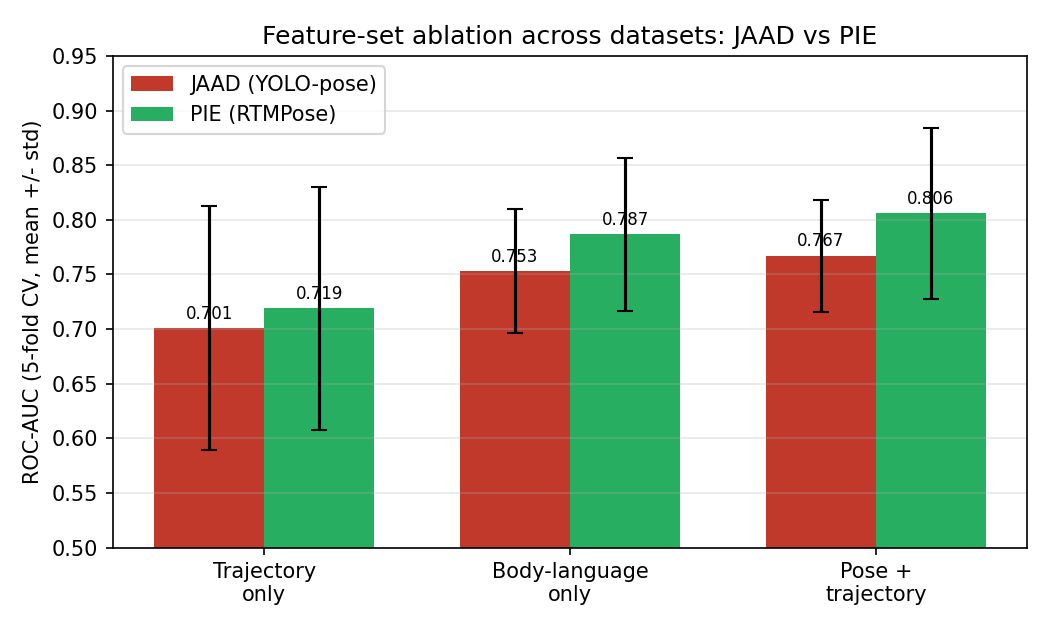
\includegraphics[width=0.48\textwidth]{jaad_pie_auc.png}
    \caption{ROC-AUC (5-fold CV, mean $\pm$ std) of the trajectory-only,
    pose-only, and pose$+$trajectory models on JAAD and PIE. The fusion model
    is best on both datasets, and the pose-based models show lower cross-fold
    variance.}
    \label{fig:jaad_pie_auc}
\end{figure}

% =====================================================================
%  QUALITATIVE VALIDATION ON INDIAN ROADS (manual video + IDD)
%  Insert as its own subsection in Results. Figures: copy the PNGs from
%  results_pie/indian_demo/ and results_pie/idd_demo/ next to the .tex.
% =====================================================================
\subsection{Qualitative Validation on Indian Roads}

To assess real-world transfer beyond the curated Western benchmarks, the
\emph{complete JAAD-trained pipeline was applied without any retraining or
fine-tuning} to Indian traffic, using two independent sources: a manually
recorded dashcam video and the Indian Driving Dataset (IDD)~[16].

\textbf{Manual dashcam video.} A 6-minute clip ($848\times478$, 29.9\,fps,
10{,}867 frames) recorded on Indian roads was processed end-to-end. RT-DETR with
ByteTrack produced \textbf{2{,}045 tracks (935 pedestrian, 1{,}110 vehicle)};
RTMPose attached 17-keypoint skeletons to \textbf{2{,}999} pedestrian detections;
the JAAD-trained LSTM produced \textbf{908 crossing-intent frame-detections}, and
the safety tagger flagged \textbf{1{,}126 of 2{,}174} processed frames as
\textsc{danger}. As no crossing-intent ground truth exists for in-the-wild
footage, this is a \emph{qualitative} demonstration of cross-domain transfer;
representative annotated frames are shown in Fig.~\ref{fig:indian_manual}. The
model correctly maintains identities and flags pedestrians stepping into the
carriageway despite unstructured traffic, mixed vehicle types, and lighting
unlike anything in the JAAD training distribution.

\textbf{Indian Driving Dataset (IDD).} As a further test of the perception front
end on Indian urban scenes, RT-DETR detection and RTMPose keypoints were run
\emph{per frame} on IDD images. IDD provides pixel-level semantic segmentation
but \emph{no} pedestrian crossing-intent labels, and its released frames are
temporally non-contiguous; it therefore supports only qualitative
detection-and-pose evaluation, not the temporal intent prediction that requires
continuous tracks. Fig.~\ref{fig:idd} shows the detector and pose estimator
generalising to dense, heterogeneous Indian traffic with up to ten pedestrians
per frame. Together these results indicate that both the perception front end and
the intent model transfer to Indian road conditions without domain-specific
retraining, supporting the pipeline's practical applicability.

\begin{figure}[t]
    \centering
    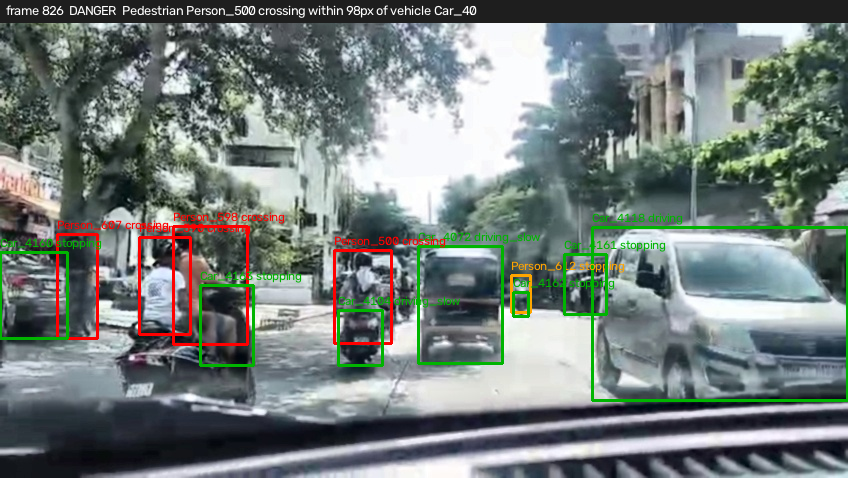
\includegraphics[width=0.48\textwidth]{indian_demo/frame_000826.png}
    \caption{JAAD-trained pipeline on a manually recorded Indian-roads video (no
    retraining): RT-DETR + ByteTrack + RTMPose + LSTM intent. Red = pedestrian
    flagged crossing/danger, orange = pedestrian safe, green = vehicle.}
    \label{fig:indian_manual}
\end{figure}

\begin{figure}[t]
    \centering
    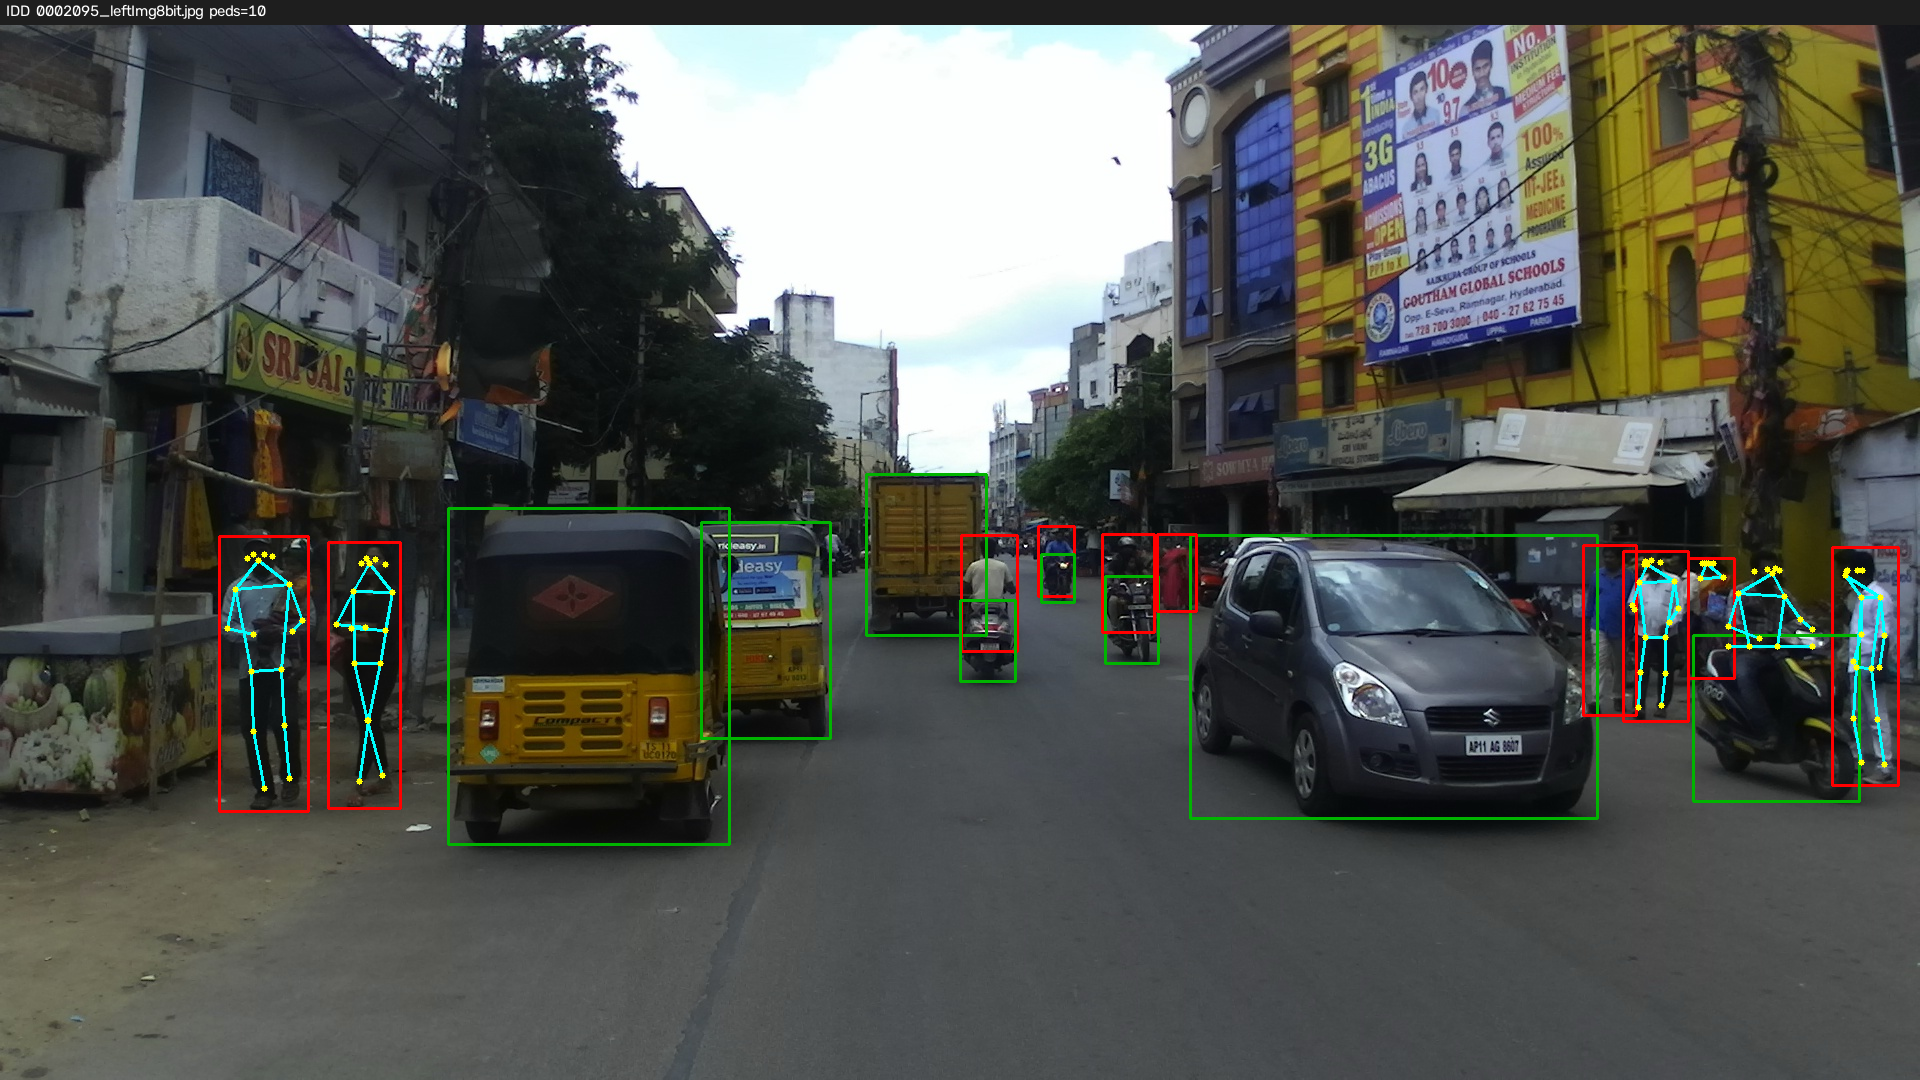
\includegraphics[width=0.48\textwidth]{idd_demo/idd_0.png}
    \caption{Perception front end (RT-DETR detection + RTMPose 17-keypoint
    skeletons) on the Indian Driving Dataset (IDD). Per-frame only: IDD frames
    are non-contiguous, so tracking and temporal intent are not applicable.}
    \label{fig:idd}
\end{figure}
